\chapter{Design and Implementation}
\label{chap:DesignImplementation}




\section{100 declarations}

evidence for equality is a coercion

% https://youtu.be/kyI9fjtgN7w?si=tsS5dSP8uguYxQxW

residual constraint - can't do any more

Any other constructs that bump levels?
% https://youtu.be/kyI9fjtgN7w&t=5353

too :: sii -> sii
too = let kuu = let muu = let zuu = let fuu = id in id in id in id in id

generalization happens in the right part
need to decide which variables to generalize over

\section{type inference as constraint solving}

type errors must contain solved variables, not just unification variables
% https://youtu.be/-TJGhGa04F8?si=rhNZurIm21c8hMi4&t=3151


floating out not described
% https://youtu.be/-TJGhGa04F8?si=nqZtTl2LdJyU3IoG&t=3312
is it really a thing?

solve simple constraints on the fly
a ~ Int
% https://youtu.be/-TJGhGa04F8?si=xVy7JRzhvL8o0EgF&t=3375

\section{generalization}

% https://www.youtube.com/watch?v=z4oShEvk3e8

\section{Solving constraints during type inference}

Implication constraints may appear without classes
% https://youtu.be/OISat1b2-4k&t=1282

% f2 = \x -> ((\y -> x) :: forall a. a -> a)

% generates

a[1] ~ beta[1] -> gamma[1]
forall a[2]. {} => gamma[1] ~ a[2]

% https://youtu.be/OISat1b2-4k?si=V6ttW72QwSTVpHQ8&t=1703

Limitation - type-directed name disambiguation (record field access)
Need partial solutions before that


\section{Remy}

% Calls them ranks

% Instead, it suffices to maintain, at every let frame and at the outermost level, a list of the type variables that are bound at this point and, conversely, to annotate every type variable in dtvÑSÖ with an integer rank, which allows telling, in constant time, where the variable is bound: type variables of rank 0 are bound at the outermost level, and type variables of rank k ≥ 1 are bound at the kth let frame down in the stack S. The code that accompanies this chapter adopts this convention. Ranks were initially described in Rémy (1992a) and have also been studied by McAllester (2003).

\section{implication constraints}

% implication constraints check for the skolem escape.
% https://github.com/ghc/ghc/blob/ed38c09bd89307a7d3f219e1965a0d9743d0ca73/compiler/GHC/Tc/Gen/Bind.hs#L1774

\section{constraint solving monad}

% data TcSEnv
% https://github.com/ghc/ghc/blob/ed38c09bd89307a7d3f219e1965a0d9743d0ca73/compiler/GHC/Tc/Solver/Monad.hs#L963


% tcs_unif_lvl

\section{Why french approach}

https://aosabook.org/en/v2/ghc.html

% > Type Checking the Source Language

\section{Levels}

we create an implication constraint at each forall

we generalize over metavariables with an ambient level (after skolemization)
% https://youtu.be/OISat1b2-4k&t=1411

% Why need promotion?
% https://youtu.be/OISat1b2-4k&t=1403

% Note [Recipe for checking a signature]
% https://github.com/ghc/ghc/blob/ed38c09bd89307a7d3f219e1965a0d9743d0ca73/compiler/GHC/Tc/Gen/HsType.hs#L206
% seems to explain things

% need to bump TcLevel on let
% Note [Inferring the type of a let-bound variable]
% https://github.com/ghc/ghc/blob/ed38c09bd89307a7d3f219e1965a0d9743d0ca73/compiler/GHC/Tc/Solver.hs#L794


% Note [Skolemisation overview]


% Does let with an annotation produce implication constraints?

% Where is TcLevel increased?
% pushTcLevel
% pushTcLevelM

% search pushTcLevelM

% Unsolved constraints
% https://github.com/ghc/ghc/blob/ed38c09bd89307a7d3f219e1965a0d9743d0ca73/compiler/GHC/Tc/Solver.hs#L328

% Various constraint types here
% Note [Canonical equalities]
% explains invariants of such equalities
% https://github.com/ghc/ghc/blob/ed38c09bd89307a7d3f219e1965a0d9743d0ca73/compiler/GHC/Tc/Types/Constraint.hs#L240


% Let should not be generalized:
% let ~ GADT

% Essence of ML
% generate, then solve constraints

% OutsideIn
% implication constraints

% Kind inference technical supplement
% level numbers

% Eisenberg talk https://www.youtube.com/live/HT8nLo6DTao
% level numbers

% let f = λx : T₁. (let g = λy : T₂. x y in g)   -- T₁ = T₂ → T₃
% in ...

% -- x : T₂ → T₃
% -- g : T₂ → T₃
% -- f : ∀ T₂, T₃. (T₂ → T₃) → T₂ → T₃


% Note [Unification preconditions]
% https://github.com/ghc/ghc/blob/ed38c09bd89307a7d3f219e1965a0d9743d0ca73/compiler/GHC/Tc/Utils/Unify.hs#L2589

% https://github.com/ghc/ghc/blob/ed38c09bd89307a7d3f219e1965a0d9743d0ca73/compiler/GHC/Tc/Solver.hs#L433
% TL;DR: bump the `TcLevel` when creating the nested implication.

% need to 
% https://www.youtube.com/live/HT8nLo6DTao?t=99m34s
% outer x    = () where
%       \a:1
%   inner y = [x;y]
%         \b:2
% 
% a:1 ~ b:2
% 
% b := a

% see Note [Use level numbers for quantification]
% "This works because we bump the level every time we go inside a new
% source-level construct."



% TODO href with texttt

\section{Core optimization}

% https://youtu.be/DiKjWl9xnvw?si=LBSpngcurBiOmeZU

\section{Questions}

1. do we keep the required type (from the annotation)?
1. Do we replace it with a more general type?

It seems like we instantiate all bound variables
% That is, we first instantiate σreq with skolem constants, and then choose how to instantiate σoff to make it match.

% in instantiate
create a type { vars :: Maybe [TcTyVar], ty :: RnType}

% Who wrote about levels?
% Implement an efficient (and language-agnostic) level-based `let`-generalization à la Rémy [^8].
% https://github.com/evermake/free-foil-typecheck/blob/ac95e6bdb440eaad7a77fd6ea0f86ef812c833e4/README.md?plain=1#L13

GHC does not have HasCallStack everywhere. Why?

\section{Technical Constraints}
\label{chap:LiteratureReview:sec:AstRepresentations:TechnicalConstraints}

My design and implementation choices were guided by the following technical constraints and requirements:

\begin{itemize}
  \item \textbf{Extensibility:} I anticipated future extensions to the language, including support for modules, integer and floating-point numbers, and record types. The chosen AST representation should accommodate such additions gracefully.
  \item \textbf{Mutual Recursion:} A requirement was the ability to employ mutually recursive data types for different categories of AST nodes. For instance, categories like modules and statements might be mutually dependent: a module could contain statements, and a statement could potentially introduce a nested module.
  \item \textbf{Annotation for Tooling:} The language server necessitated annotating AST nodes with auxiliary information. This includes the source code location (span) corresponding to each node and the inferred type of the expression represented by a node's subtree.
  \item \textbf{Parser Generator Integration:} I utilized the BNFC parser generator \cite{bnfc-site-2025}.
\end{itemize}


% TODO mention which ones are a solution to the expression problem and if it was relevant in our case.

% TODO Evaluate approaches?

\section{TTG}

TTG is mostly orthogonal to other approaches.
It does not try to reuse existing functions, but rather allows to reuse existing data type declarations.
Extension fields are for fields that occur not in all versions of the AST.



The parsers generated by BNFC do not directly support parsing signed integer literals. A common workaround involves defining a custom \texttt{token} for the pattern, parsing it into a node containing the raw string representation, and subsequently post-processing the generated AST to convert these string-based nodes into nodes containing the actual numeric values using an \texttt{internal} (non-parsable) constructor.

\begin{minted}{haskell}
token IntegerSigned ('-'? digit+) ;
-- Node holding the raw string
LitIntegerRaw. Object ::= IntegerSigned ;
-- Node holding the parsed Integer
internal LitInteger. Object ::= IntegerSigned ;
\end{minted}

A drawback of this approach is the persistence of both node variants (\texttt{LitIntegerRaw} and \texttt{LitInteger}) within the AST data type definition. This requires handling the \texttt{LitIntegerRaw} case in pattern matching, even though it becomes redundant after the post-processing step.



Initially, I considered using the Free Foil representation of my AST to track bound variables. However, I later found out that the Free Foil approach presented two potential limitations relative to my technical constraints (\cref{chap:LiteratureReview:sec:AstRepresentations:TechnicalConstraints}):

First, the current library version requires mutually recursive types within the AST to be combined into a single sum data type acting as the signature \texttt{sig}. The library author notes that supporting truly separate mutually recursive types might be theoretically possible using a different internal representation.

% TODO link to the definition of lexical scoping
Second, Free Foil might increase the AST complexity or size in the version of PLC featuring modules or other forms of non-lexical scoping. For instance, in a language with modules, correctly relating variable declarations to their usage sites might necessitate multi-phase analysis (e.g., using scope graphs \cite{poulsen-monadic-2023}). If binders are used to track declaration sites, one might need to: (1) parse into an initial AST without resolved binders, (2) perform scope analysis, and (3) construct the second AST with appropriate binders reflecting the resolved scopes. For module imports, this could involve adding nodes within the import's subtree that introduce binders for all imported symbols, while simultaneously needing to retain information about the originating module for each binder.

% Unlike the current Free Foil implementation, Trees That Grow readily supports mutually recursive data types. Its usage pattern resembles employing standard parameterized algebraic data types, although it necessitates defining a significant number of type family instances for constructor fields.


Key techniques adopted from GHC included utilizing the Trees That Grow (TTG) \cite{trees-that-grow-2016} abstract syntax tree (AST) representation, supporting parametric predicative higher-rank polymorphism \cite{jones-practical-2007}, implementing a bidirectional constraint collection algorithm \cite{jones-typechecker-2023}, having a separate constraint solver \cite{jones-typechecker-2023}, translating the source language to a System F-based core language (Core) \cite{jones-practical-2007}, inlining \cite{jones-rapier-2002} and evaluating this Core.

Additionally, I investigated available options for the AST representation and type inference engine to inform my design choices. For example, I studied the Free Foil approach \cite{kudasov-free-2024}, which enabled type-safe capture-avoiding substitution for the Core.

To facilitate rapid iteration on the language syntax, I chose the BNFC parser generator \cite{bnfc-parser-generator} rather than the combination of Happy and Alex employed by GHC \cite{ghc-gitlab-2025}.

The accompanying Technical Appendix \cite{practical-type-inference-proofs} provides proofs of soundness and completeness for the theoretical system described in the paper, but not for the attached Haskell implementation.

% -- need parens in type checking

% forall a. a -> a
% (forall a. a -> a) -> a


% <!-- Evaluation of the recipe -->
% How many lines for type checker in GHC?
% How many lines in my implementation?
% Comment lines?


% # Results

% 1. Generated a parser for STLC using the BNFC parser generator [BNFC].
% 1. Represented the annotated language AST using the Trees That Grow approach [SPJ, TTG].
% 1. Adapted the bidirectional algorithm from [SPJ, Practical] for type constraints collection.
% 1. Implemented type inference via standalone constraint solver [Jones, 100 types] using levels [Eisenberg, WITS].
% 1. Added type-directed translation of the typechecked AST to the Core language [SPJ, Practical].
% 1. Replaced the rapier approach [SPJ, Secrets] with Free Foil to enable scope-safe Core transformations.
% 1. Implemented one inlining optimization on the Core language [SPJ, Rapier].
% 1. Provided the Core expressions evaluator.
% 1. Developed a language server.


\section{Architecture}
\label{chap:DesignImplementation:sec:Architecture}

\subsection{Static view}

\newpage

\begin{figure}[h]
  \centering
  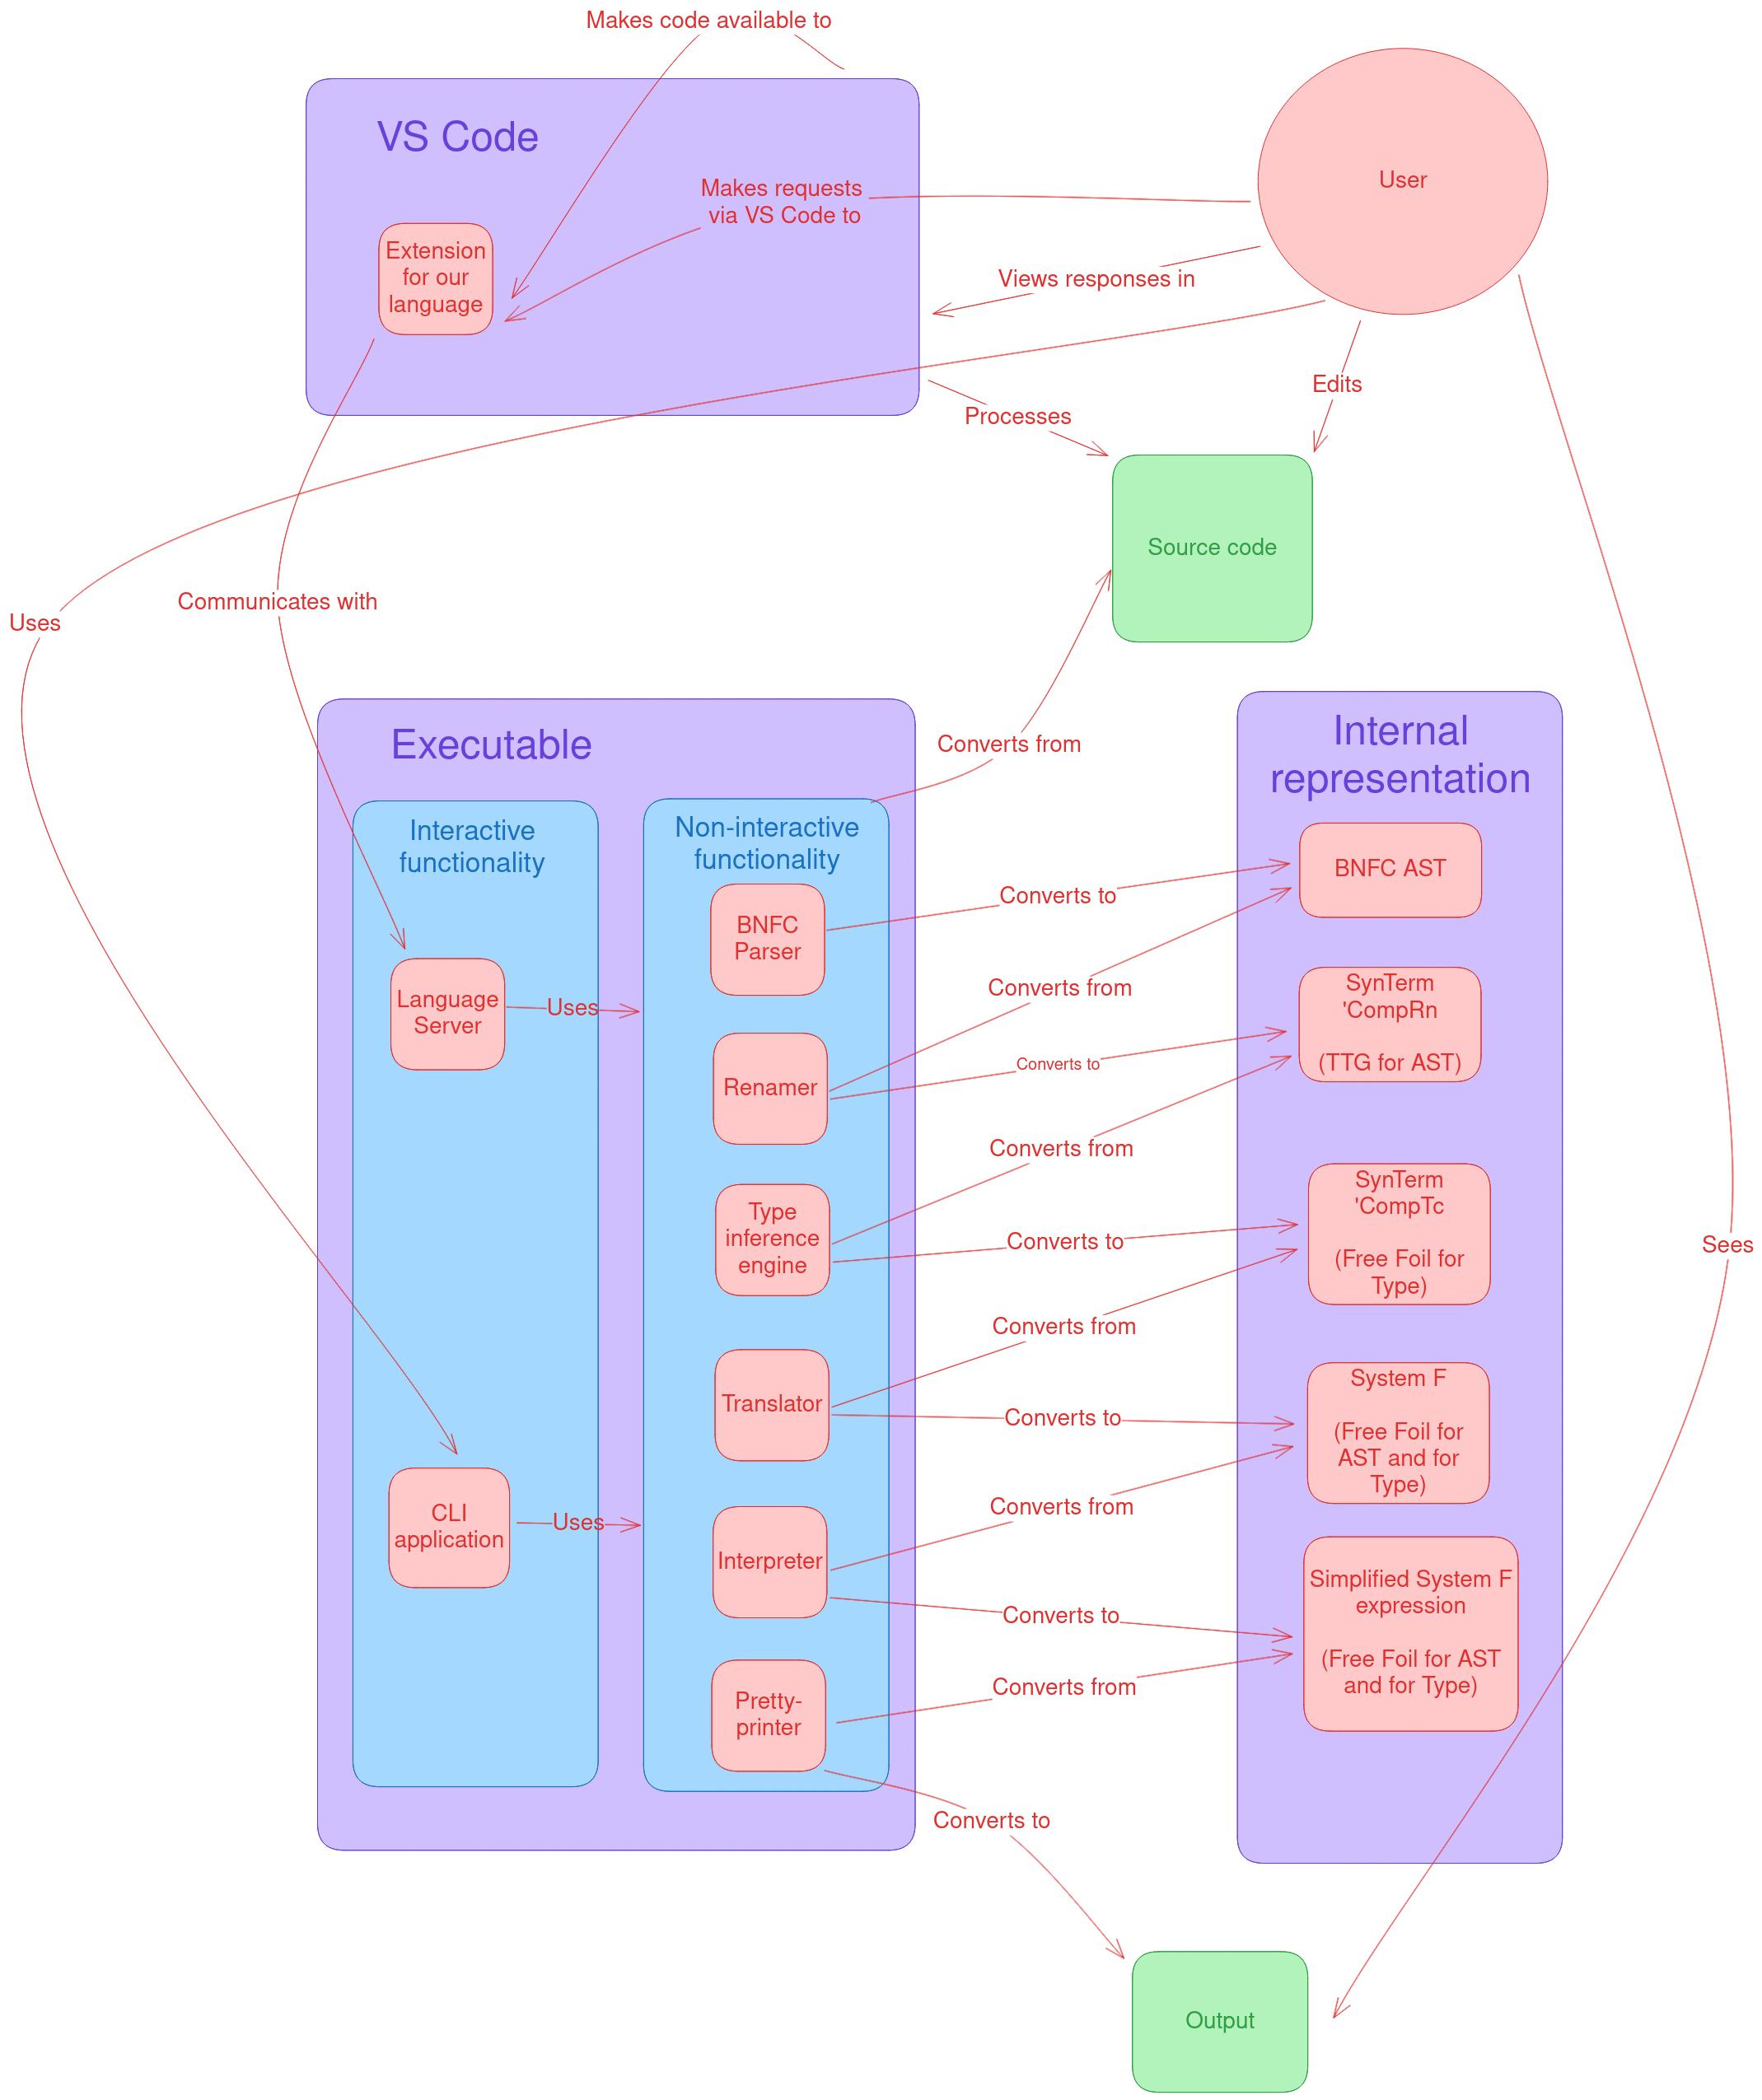
\includegraphics[scale=0.25]{Architecture.png}
  \caption{Static view}
  \label{Architecture}
\end{figure}

\newpage

\subsection{Use Case: Interpreter is called.}

\subsubsection{Parsing}

A BNFC-generated parser reads the source code written in my language and produces a raw BNFC AST with positions of tokens.

\subsubsection{Renaming}

The raw BNFC AST is then converted to the Trees That Grow representation \texttt{SynTerm 'CompRn}.
During conversion, positions are copied to annotations and each variable in the program gets a unique identifier under condition.
Same variables appearing in multiple places in the program get the same identifiers.

\subsubsection{Typing}

The typing algorithm runs.
It uses the Free Foil representation of Core Types.
The typing algorithm annotates the tree with fully instantiated (not having metavariables) types producing \texttt{SynTerm 'CompTc} or throwing an error.

\subsubsection{Translation to System F}

The \texttt{SynTerm 'CompTc} is converted to the System F syntax using the Free Foil representation.

\subsubsection{Interpretation}

The interpreter evaluates the System F code.

\subsubsection{Output}

The program pretty-prints the resulting expression.

\subsection{Use case: user queries a type of a variable.}

\subsubsection{Start language server}

VS Code extension starts the language server if not started.
VS Code extension makes the language server read the code in the current file.

\subsubsection{Query}

VS Code extension passes a position to the language server and asks for the type of the variable at that position.

\subsection{Process}

The language server updates the AST if necessary, performs type checking, finds the node at the given position, and returns its type to the extension.

\section{AST}

I used the Trees That Grow approach \cite{trees-that-grow-2016} for the AST representation.

In GHC, some fields are just types constructed using the index parameter. In contrary, I used type family applications to the index parameter in all fields of the AST to make the AST more flexible. Additionally, I named the type families and constructors consistently to improve code navigation.

\begin{minted}{haskell}
-- GHC

-- Language/Haskell/Syntax/Expr.hs

data HsExpr p
  = HsVar     (XVar p)
              (LIdP p)
    ...

-- Language/Haskell/Syntax/Extension.hs

type LIdP p = XRec p (IdP p)

-- Ours

-- Language/STLC/Typing/Jones2007/BasicTypes.hs

data SynTerm x
    = -- | variables
      SynTerm'Var (XSynTerm'Var' x) (XSynTerm'Var x)
    ...

-- The Name already contains an SrcSpan, so it does not need an annotation
type instance XSynTerm'Var x = Name
\end{minted}

Like in GHC, I had separate data types that represented syntactic types and types used during typing.

\begin{minted}{haskell}
-- Ours

-- Language/STLC/Typing/Jones2007/BasicTypes.hs

data SynType x
  = -- | Type variable
    SynType'Var (XSynType'Var' x) (XSynType'Var x)
    ...

data Type
  = -- | Vanilla type variable.
    Type'Var Var
  ...
\end{minted}

\section{Type system}

A \textit{type system} specifies syntactic rules of assigning types to terms (e.g., expressions, operators, statements) of a program written in a programming language, allowing one to reason about the run-time properties of that program \cite{pierce-types-2002}.
A \textit{bidirectional} type system has some rules that infer and some rules that check types of terms \cite{dunfield-bidirectional-2020}.

\cref{chap:DesignImplementation:sec:GhcTypecheckingError} informally explains the basic GHC type checking principles using a Haskell program that fails to type check.
\cref{chap:DesignImplementation:sec:VslTypeSystem} describes a slightly revised version of the bidirectional type system suggested by \citeauthor{jones-practical-2007} \cite[Sec. 4.7]{jones-practical-2007} that I implemented in my calculus.


% TODO why need this to be a subsection of the `Type system' section?
\subsection{GHC typechecking principles}
\label{chap:DesignImplementation:sec:GhcTypecheckingError}

This section informally explains the basic GHC type checking principles using Haskell programs that fail to type check.

\subsubsection{Example 1}

Consider the following program.

\begin{minted}{haskell}
{-# LANGUAGE RankNTypes #-}

poly :: forall a. (forall s. s) -> a
poly = undefined
\end{minted}

The GHC typechecker produced the following error on this code:

\begin{minted}{text}
• Couldn't match expected type ‘(forall s. s) -> a’
  with actual type ‘a0’
  Cannot instantiate unification variable ‘a0’
with a type involving polytypes: (forall s. s) -> a
• In the expression: undefined
  In an equation for ‘poly’: poly = undefined
\end{minted}

Why did typechecking fail?

\subsubsection{Explanation (Example 1)}

% TODO caption

% TODO why a -> b works? does not it have an implicit forall?
% only types where all foralls can be moved to the left work?

During typechecking, GHC infers types of unannotated terms.
Initially, the compiler does not know these types, so it creates named placeholders for these types called unification variables or metavariables (see \href{https://gitlab.haskell.org/ghc/ghc/-/wikis/Zonking}{Zonking}, \href{https://github.com/ghc/ghc/blob/ed38c09bd89307a7d3f219e1965a0d9743d0ca73/compiler/GHC/Types/Var.hs#L169}{\texttt{GHC.Types.Var}}).
These unification variables have a mutable field where the resolved type can later be written.
That type is resolved via unification, hence the name "unification variables".

Before unification, GHC collects various constraints on types, e.g. that certain pairs of types are equal.
GHC solves such constraints one by one.
If a constraint states that two types are equal, GHC tries to unify them.
GHC inspects corresponding parts of these two types, e.g., the types of the first arguments and the types of results.
If GHC sees a metavariable in one of the types, it equates that metavariable with the corresponding part of another type.
If that part contains metavariables, GHC adds this new equation to its list of constraints and tries to solve that constraint later.
% TODO is this true?
On the other hand, if that part does not contain metavariables, GHC writes the type represented by that part into the metavariable and marks that metavariable resolved (zonked).
% TODO proof
After GHC resolves all constraints, it writes \texttt{Any} types into the remaining metavariables.

% TODO need to unify with monotypes to be able to solve in arbitrary order
As explained in \cite{jones-practical-2007}, during unification, metavariables must always be equated with monotypes, i.e. types without \texttt{forall} anywhere.
% TODO we don't have deep instantiation? Maybe deep skolemise?
% TODO does it instantiate any metavariables before unification introduced in that \texttt{forall} with non-metavariables

If GHC can move all \texttt{forall}s to the left of the type, it will do so before unification.
So, \texttt{forall a. a -> (forall s. s)} will be transformed into \texttt{forall a s. a -> s}.

% TODO reference to the example
In the example above, GHC created a metavariable \texttt{a0} standing for the type of \texttt{undefined}.
Next, it tried to unify \texttt{a0} with the type \texttt{forall a. (forall s. s) -> a} given in the signature of \texttt{poly}.
That type is a polytype, i.e., a type containing a \texttt{forall}.
Moreover, it is a higher-rank type, that is, it has a \texttt{(forall s. s)} to the left of the function arrow.
So, it is impossible to move the \texttt{forall} outside of the parenthesis because the \texttt{(forall s. s)} is not a return type inside \texttt{forall a. (forall s. s) -> a}.
Therefore, the unification failed.

\subsubsection{Example 2}

Consider the following program.

\begin{minted}{haskell}
{-# LANGUAGE RankNTypes #-}

poly1 x = (x 42, x "Hello")
\end{minted}

The GHC typechecker produced the following error on this code:

\begin{minted}{text}
• Couldn't match type ‘[Char]’ with ‘Bool’
  Expected: Bool
    Actual: String
• In the first argument of ‘x’, namely ‘"Hello"’
  In the expression: x "Hello"
  In the expression: (x True, x "Hello")
\end{minted}

Why did typechecking fail?

\subsubsection{Explanation (Example 2)}

In this case, there are no type annotations.
Hence, GHC created a unification variable for \texttt{x}.
It also created a couple of constraints with that metavariable.
First, \texttt{x} is a function with a type \texttt{Bool -> a}.
Second, \texttt{x} is a function from \texttt{String -> b}.
Then, it unified the metavariable with \texttt{Bool -> a}.
Next, it started processing the second constraint and tried to unify \texttt{Bool -> a} with \texttt{String -> b}.
However, \texttt{Bool} and \texttt{String} are incompatible.
Therefore, typechecking failed.

% TODO example NoMonoLocalBinds
% https://dl.acm.org/doi/abs/10.1145/1708016.1708023

\section{VSL type system}
\label{chap:DesignImplementation:sec:VslTypeSystem}

% > Haskell implements the Damas-Milner rule that a lambda-bound argument (such as x) can only have a monomorphic type.
% Does the new system support polymorphic lambda arguments?
% > Notice the programmer-supplied type signature for f, which expresses the polymorphic type of f’s argument.
% Seems like yes if we assume f is a lambda

what are higher rank types?

\newpage

% TODO improve the alignment

\newcommand{\Qquad}{\hspace{0.25em}}
\newcommand{\mexp}[1]{\mathnormal{#1}}
\newcommand{\msyn}[1]{\normalfont\asciifamily\text{#1}}
\newcommand{\mlg}[1]{\mathlarger{\mathlarger{#1}}}

\begin{figure}[h]
  \begin{tcolorbox}[breakable, colback=white]
    \small
    % Using gather* to center each rule or pair of rules on a line
    \begin{gather*}
      \mlg{\text{Rho-types} \quad \rho \Qquad \Coloneqq \Qquad \tau \mid \sigma \to \sigma}
      \\[\bigskipamount]
      \boxed{\mlg{\Gamma \vdash_\delta \mexp{t} : \rho}} \qquad \delta \Coloneqq \Qquad \Uparrow \Qquad \mid \Qquad \Downarrow
      \\[\bigskipamount]
      \frac{}{\Gamma \vdash_\delta \mexp{i} : \msyn{Int}} \text{INT}
      \qquad \qquad
      \frac{\mexp{\vdash_\delta^{inst} \sigma \leq \rho}}{\Gamma, \mexp{(x:\sigma) \vdash_\delta x : \rho}} \text{VAR}
      \\[\bigskipamount]
      \frac{\Gamma, \mexp{(x:\tau) \vdash_\Uparrow \mexp{t} : \rho}}{\Gamma \Qquad \mexp{\vdash_\Uparrow (\lambda x.t) : (\tau \to \rho)}} \text{ABS1}
      \qquad \qquad
      \frac{\Gamma, \mexp{(x:\sigma_a) \vdash_\Downarrow^{poly} t : \sigma_r}}{\Gamma \Qquad \mexp{\vdash_\Downarrow (\lambda x.t) : (\sigma_a \to \sigma_r)}} \text{ABS2}
      \\[\bigskipamount]
      \frac{\Gamma, \mexp{(x:\sigma) \vdash_\Uparrow t : \rho}}{\Gamma \Qquad \mexp{\vdash_\Uparrow (\forall x \msyn{::} \sigma).t : (\sigma \to \rho)}} \text{AABS1}
      \\[\bigskipamount]
      \frac{\mexp{\vdash^{dsk} \sigma_a \leq \sigma_x} \quad \Gamma, \mexp{(x:\sigma_x) \vdash_\Downarrow^{poly} t : \sigma_r}}{\Gamma \Qquad \mexp{\vdash_\Downarrow (\forall x \msyn{::} \sigma_x).t : (\sigma_a \to \sigma_r)}} \text{AABS2}
      \\[\bigskipamount]
      \frac{\Gamma \Qquad \mexp{\vdash_\Uparrow t : (\sigma \to \sigma')} \quad \Gamma \Qquad \mexp{\vdash_\delta^{poly} u : \sigma \quad \vdash_\delta^{inst} \sigma' \leq \rho}}{\Gamma \Qquad \mexp{\vdash_\delta t \Qquad u : \rho}} \text{APP}
      \\[\bigskipamount]
      \frac{\Gamma \Qquad \mexp{\vdash_\delta^{poly} t : \sigma \quad \vdash_\delta^{inst} \sigma \leq \rho}}{\Gamma \Qquad \mexp{\vdash_\delta (t \msyn{::} \sigma) : \rho}} \text{ANNOT}
      \qquad
      \frac{\Gamma \Qquad \mexp{\vdash_\delta^{poly} u : \sigma} \quad \Gamma, \mexp{x:\sigma \vdash_\delta t : \rho}}{\Gamma \vdash_\delta \msyn{let} \Qquad \mexp{x} \Qquad = \Qquad \mexp{u} \Qquad \msyn{in} \Qquad \mexp{t : \rho}} \text{LET}
      \\[\bigskipamount]
      \boxed{\mlg{\Gamma \Qquad \mexp{\vdash_\delta^{poly} t : \sigma}}}
      \\[\bigskipamount]
      \frac{\mexp{\bar{a}} = \mexp{ftv}(\rho) - \mexp{ftv}(\Gamma) \quad \Gamma \Qquad \mexp{\vdash_\Uparrow t : \rho}}{\Gamma \Qquad \mexp{\vdash_\Uparrow^{poly} t : \forall \bar{a}.\rho}} \text{GEN1}
      \\[\bigskipamount]
      \frac{\mexp{\bar{a}} \notin \mexp{ftv}(\Gamma) \quad \Gamma \Qquad \mexp{\vdash_\Downarrow t : \rho \quad pr(\sigma) = \forall \bar{a}.\rho}}{\Gamma \Qquad \mexp{\vdash_\Downarrow^{poly} t : \sigma}} \quad \text{GEN2}
      \\[\bigskipamount]
      \boxed{\mlg{\mexp{\vdash_\delta^{inst} \sigma \leq \rho}}}
      \\[\bigskipamount]
      \frac{}{\mexp{\vdash_\Uparrow^{inst} \forall \bar{a}.\rho \leq [a \mapsto \tau] \rho}} \text{INST1}
      \qquad \qquad
      \frac{\mexp{\vdash^{dsk} \sigma \leq \rho}}{\mexp{\vdash_\Downarrow^{inst} \sigma \leq \rho}} \text{INST2}
    \end{gather*}
  \end{tcolorbox}
  \caption{Bidirectional type system}
  \label{fig:TypeSystem}
\end{figure}

\section{TODO}

TODO use the Free Foil representation for Type
TODO Free foil - try to marry with indices assigned by the Tc monad
TODO write about the type system.

\section{Core AST representation}

\subsection{Foil + \texttt{hypertypes} + \texttt{free-foil}}

It is possible to combine the \texttt{Foil} (\cref{chap:LiteratureReview:sec:AstRepresentations:Foil}), \texttt{hypertypes} (\cref{chap:LiteratureReview:sec:AstRepresentations:Hypertypes}), and \texttt{Free Foil} (\cref{chap:LiteratureReview:sec:AstRepresentations:FreeFoil}) approaches to support scoped mutually recursive types.

% TODO break page?

\begin{minted}{haskell}
  type H = AHyperType
  type BinderType = S -> S -> Type
  type ExprType = S -> H -> Type
  
  data H'Var (n :: S) (h :: H)
    = H'Var {_varName :: (Name n)}
  
  data
    H'Lam
      (binder :: BinderType) (expr :: ExprType)
      (n :: S) (h :: H)
    = forall (l :: S).
    H'Lam
    { _lamBinder :: binder n l
    , _lamExpr :: h :# expr l
    }
  
  data
    H'App
      (funcExpr :: ExprType) (argExpr :: ExprType)
      (n :: S) (h :: H)
    = H'App
    { _appFunc :: h :# funcExpr n
    , _appArg :: h :# argExpr n
    }
  
  data H'Exp (n :: S) h
    = H'Exp'Var (H'Var n h)
    | H'Exp'Lam (H'Lam NameBinder H'Exp n h)
    | H'Exp'App (H'App H'Exp H'Exp n h)
\end{minted}

% perform typing on a slightly desugared AST.
% I used the Free Foil representation of the Core types.

% TODO schema

% Free foil - try to marry with indices assigned by the monad